\documentclass[11pt]{article}
\usepackage[utf8]{inputenc}
\usepackage[russian]{babel}
\usepackage[T1]{fontenc}
\usepackage{amssymb,amsmath,clrscode,graphicx,indentfirst}

\author{Олег Смирнов}
\title{Курс kiev-clrs -- Лекция 9. Двоичные поисковые деревья}
\date{31 мая 2009 г.}

\begin{document}
\maketitle
\tableofcontents

\newpage
\setlength{\parskip}{1ex plus 0.5ex minus 0.2ex}
\section{Цель лекции}
\begin{itemize}
\item 
\item 
\item 
\end{itemize}

\section{Бинарные деревья поиска}

``Хорошими'' считаются сбалансированные бинарные деревья с высотой порядка $O(\lg n)$. У несбалансированных бинарных деревьев высота может достигать $n$. Время прохода по бинарному дереву пропорционально его высоте. Цель -- построить бинарное дерево с высотой порядка $O(\lg n)$ в большинстве случаев. Один из способов -- рандомизация, рассматривается в данной лекции.

\subsection{Сортировка массива}

Бинарные деревья поиска (Binary search tree, BST) можно использовать для сортировки массива:
\begin{codebox}
\li $T \gets \emptyset $
\li \For $i \gets 1$ \To $n$
\li \Do Tree\_Insert($T$, $A[i]$)
  \End
\li Inorder\_Tree\_Walk(root$[T]$)
\end{codebox}

\begin{figure}[ht]
  \centering
  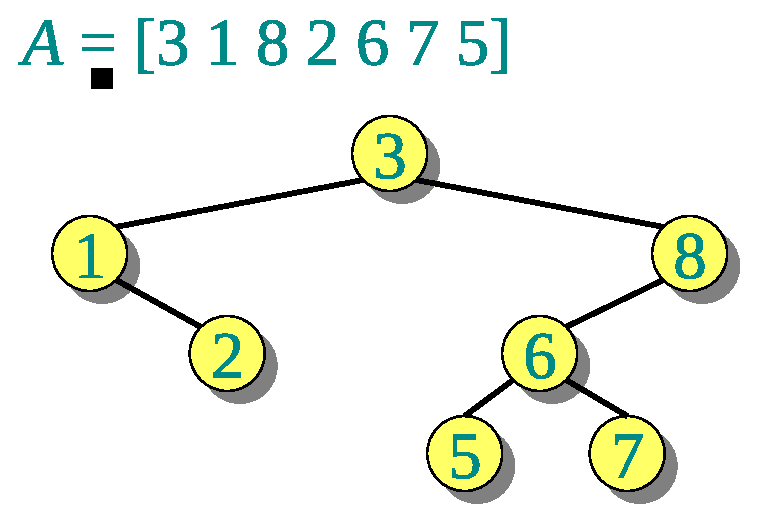
\includegraphics[width=2in]{lecture9/bs_tree.eps}
  \caption{Дерево работы BST sort}
  \label{fig:bs_tree}
\end{figure}

Время работы алгоритма складывается из частей:
\begin{itemize}
\item $O(n)$ для обхода Inorder\_Tree\_Walk
\item $\Omega(n \lg n)$ для Tree\_Insert в среднем и в лучшем случае (идеально сбалансированное бинарное дерево)
\item $T = \sum_{x \in T} depth(x) = \Theta(n^2)$ для Tree\_Insert в худшем случае (массиво уже отсортирован)
\end{itemize}

Поведение алгоритма похоже на поведение сортирвки Хоара -- Quicksort.

\section{BST и сортировка Хоара}

Алгоритмы BST sort и Quicksort выполняют одинаковое количество сравнений, но в различном порядке.
\begin{figure}[ht]
  \centering
  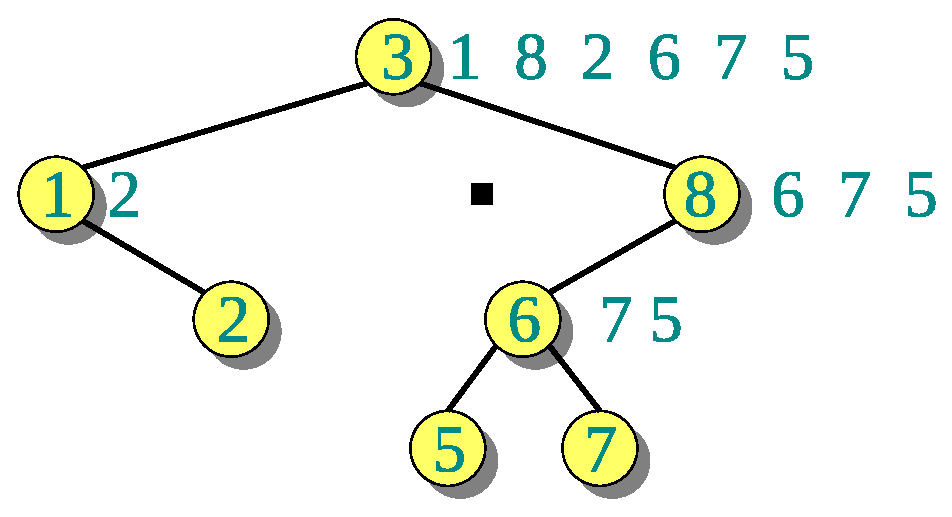
\includegraphics[width=2in]{lecture9/qs_tree.eps}
  \caption{Дерево работы Quicksort}
  \label{fig:qs_tree}
\end{figure}

Полученное дерево в точности совпадает с построенным в предыдущем примере.

Анализируя работу, можно увидеть, что алгоритм Quicksort в начале делает сравнение всех элементов с первым опорным (3), генерируя первое разбиение. BST sort также сравнивает каждый элемент в порядке добавления с корнем дерева (3). Аналогичные сравнения происходят для каждого элемента массива. Элемент, который в Quicksort становится опорным, в BST sort становится корнем поддерева.

\subsection{Рандомизированный BST sort}
\begin{enumerate}
\item Случайная перестановка элементов массива
\item Сортировка BST sort(A)
\end{enumerate}

Время работы совпадает со временем рандомизированного Quicksort. Совпадает и мат. ожидание.
\begin{equation*}
  E[\text{time}] = E[\text{Randomized\_Quicksort}] = \Theta(n \lg n)
\end{equation*}

Нет смысла использовать BST sort для сортировки массива, т.к. время не отличается от Quicksort. Поиск по BST также не дает преимуществ по сравнению с бинарным поиском в просто отсортированном массиве. Полезность BST заключается в возможности добавлять элементы в структуру динамически, при этом сохраняя ожидаемое время работы.

\section{Анализ высоты BST}


\end{document}
